% RQ4 (zone occupancy) built on its own, so it can be read and checked before
% the joint 8-page paper exists.
%
% Build:   tectonic draft_rq4.tex      (or upload paper/ to Overleaf)
% Numbers: python figures/make_figures.py   (writes figures/rq4_numbers.tex and
%          figures/rq4_zones.pdf from results/rq4_zones.json and
%          results/rq4_detection.json; a missing number prints as ??)
%
% The preamble is a copy of ifas.tex's, so the section drops into the joint
% paper unchanged.
\documentclass[conference]{IEEEtran}

\usepackage[T1]{fontenc}
\usepackage[utf8]{inputenc}
\usepackage{microtype}
\usepackage{cite}
\usepackage{amsmath,amssymb}
\usepackage{graphicx}
\usepackage{booktabs}
\usepackage{array}
\usepackage{xcolor}
\usepackage{tikz}
\usetikzlibrary{arrows.meta,chains,positioning,decorations.pathreplacing,calc}
\usepackage[hidelinks]{hyperref}

\graphicspath{{figures/}}

\definecolor{ink}{HTML}{1B1F3B}
\definecolor{cool}{HTML}{2A6FDC}
\definecolor{warm}{HTML}{E0602A}

\begin{document}

\title{RQ4: Which Seats Are Taken? Zone Occupancy from One Fixed Camera\\(draft for the research rewrite)}
\author{\IEEEauthorblockN{IFAS team}}
\maketitle

% RQ4: zone occupancy from one fixed camera.
% Every number below comes from results/rq4_zones.json and
% results/rq4_detection.json through figures/rq4_numbers.tex, which
% make_figures.py writes. A number that does not exist yet prints as ?? in bold.
% Lines marked TODO need occupancy labels (the zone labelling page) or footage
% where people actually leave.

\providecommand{\rqfour}[1]{%
  \ifcsname rq4/#1\endcsname\csname rq4/#1\endcsname\else\textbf{??}\fi}
\InputIfFileExists{figures/rq4_numbers.tex}{}{}

\section{Zone Occupancy: Which Seats Are Taken?}
\label{sec:rq4}
In a restaurant, a library or a lecture hall, the useful question is often not
\emph{who} is in view but \emph{which places are in use}, for how long, and which
will free up next. That question needs no identity and no attribute model: a
place is taken while someone is in it. We ask how reliably one fixed camera
can answer it, which design choices the answer depends on, and whether it holds
up where per-person counting does not. Our hypothesis (H4) is that occupancy is
far more robust to identity errors than footfall, because it never asks whether
two sightings are the same person.

\subsection{Method}
\emph{Zones.} A zone is a polygon in the image, a seat, a table, a queue or a
free area, drawn in the workbench or proposed automatically (below).

\emph{Where a person is.} Each detection is reduced to one point, its anchor.
For standing people the bottom centre of the box is the usual ground contact
point, but a seated person's feet are hidden behind the desk, so the default is
the point a fraction $\lambda$ of the way down the box,
$a = \big(\tfrac{x_1+x_2}{2},\; y_1 + \lambda (y_2-y_1)\big)$ with
$\lambda = 0.85$. The alternatives are the foot point, the centre, and the share
of the lower half of the box that overlaps the zone. An anchor inside several
zones goes to the smallest, so a seat drawn inside a table wins.

\emph{Spatial hysteresis.} A seated person leans, and their anchor crosses into
the neighbouring seat for a moment. With hysteresis $s$, a person placed in zone
$Z$ stays there until the anchor leaves $Z$ scaled by $1+s$ about its centroid,
or enters another zone's core, scaled by $1/(1+s)$. We use $s =
\rqfour{stick}$.

\emph{Temporal smoothing.} Per zone, raw presence on the sampling grid is cleaned
in two steps: absences shorter than $\tau_{\mathrm{off}}$ are bridged as missed
detections, then stays shorter than $\tau_{\mathrm{on}}$ are dropped as
passers-by ($\tau_{\mathrm{on}} = \rqfour{on-sec}$\,s, $\tau_{\mathrm{off}} =
\rqfour{off-sec}$\,s). Timestamps stay exact; only the reported state lags by
these amounts in a live setting. A stay that reaches either end of the recording
is right- or left-censored, and an absence cut off by the end of the recording
that is shorter than $\tau_{\mathrm{off}}$ is not counted as leaving. Without
that last rule every seat whose occupant was missed in the final seconds read
as free.

\emph{Which seat frees up next.} Stays from every seat feed one Kaplan--Meier
estimate $\hat S(t)$~\cite{kaplan1958}, with censored stays counted as lasting
at least as long as observed. For a seat taken for $e$ seconds, the expected
remaining time is the mean residual life
$m(e) = \int_e^\infty \hat S(u)\,du \,/\, \hat S(e)$, and the seat with the
smallest $m(e)$ is named next. We compare it with the rule a person would use,
\emph{taken longest}, and with chance, causally: at each moment the estimate
uses only stays that had ended by then. The workbench names the seat taken
longest and shows $m(e)$ as its expected time left.

\emph{Automatic seats.} A \emph{stay} is a stretch of at least 20\,s in which a
track's anchor moves less than a third of a body height. Stays within half a
body width of each other merge into one place, and a place becomes a seat if it
gathers at least $40$\,s of stays in total. Seats are numbered in reading order.

\emph{Detection.} Seated people far from the camera are small and half hidden by
the row in front. Besides the full frame, the detector looks at a $2\times2$
grid of tiles with 20\% overlap, and boxes are merged by non-maximum
suppression that also drops a box lying mostly inside a stronger one (a person
cut by a tile edge)~\cite{akyon2022sahi}.

\subsection{Data}
One \rqfour{duration-min}-minute recording from a ceiling camera in a lecture
room at a college, 1920$\times$1080 at 25 frames/s, with about forty students
seated in rows of benches throughout. It was processed with YOLOv8n and tiling,
sampling every \rqfour{sample-sec}\,s; the \rqfour{zones} seats were
\rqfour{zone-source}. % TODO: record the college's permission for this footage
% in docs/research-data.md before any of this is submitted.
Nobody left during the recording, which makes it a hard test of stability (the
right answer is ``taken'' almost everywhere, almost all the time) and no test of
the next-free rule. Seat occupancy was labelled on the \rqfour{lab-moments}
saved frames (\rqfour{lab-items} seat-moments, \rqfour{lab-unsure} more left
unsure) by an AI annotator, from clean frames showing only the seat outlines.
These labels are not human ground truth: they rank settings against each other,
and the numbers that rest on them are to be confirmed by two people (TODO).

\begin{figure*}[t]
  \centering
  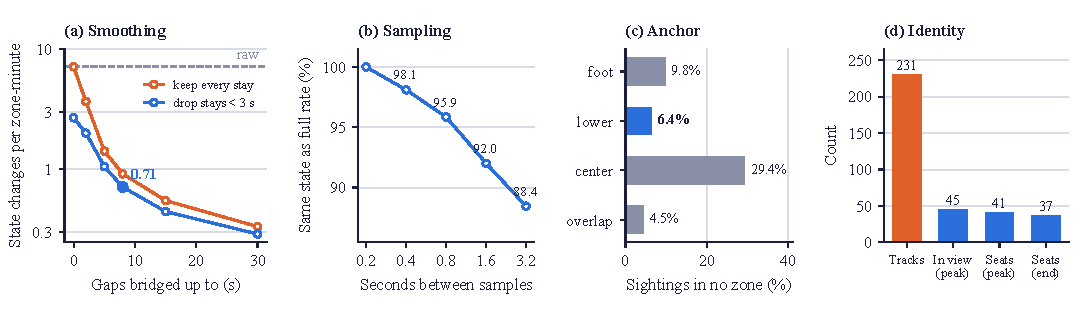
\includegraphics[width=\textwidth]{rq4_zones.pdf}
  \caption{Zone occupancy on the lecture recording. (a)~Seat-state changes per zone-minute
  against the longest gap bridged, keeping every stay or dropping those under
  3\,s; dashed: raw presence. (b)~Agreement of the smoothed state with the full
  sampling rate when the run is sampled less often. (c)~Share of sightings that
  fall in no zone, by anchor rule. (d)~Tracks against people: tracks fragment,
  occupancy does not need them to be whole.}
  \label{fig:rq4}
\end{figure*}

\subsection{Results}
\emph{Detection limits everything else.} On \rqfour{det-frames} frames spread
through the recording, YOLOv8n at its default input size finds
\rqfour{det/yolov8n/none/0.4} people per frame at confidence 0.4, and
\rqfour{det/yolov8n/2x2/0.4} with tiling; YOLOv8s finds
\rqfour{det/yolov8s/none/0.4} and \rqfour{det/yolov8s/2x2/0.4}, and YOLOv8m
\rqfour{det/yolov8m/none/0.4} and \rqfour{det/yolov8m/2x2/0.4}. Tiling costs
\rqfour{det/yolov8n/2x2/sec}\,s per frame against \rqfour{det/yolov8n/none/sec}\,s
for YOLOv8n on our CPU. These are counts, not recall: without box labels a
higher count can include false positives.

\emph{Smoothing.} Raw presence changes state \rqfour{raw-flicker} times per
zone-minute; smoothing brings that to \rqfour{flicker}, a
\rqfour{flicker-ratio}-fold reduction (Fig.~\ref{fig:rq4}a). The choice of
$\tau_{\mathrm{off}}$ matters more than $\tau_{\mathrm{on}}$, and longer bridges
keep lowering flicker while raising utilisation. Spatial hysteresis removes
\rqfour{stick-cut}\% of the raw changes (\rqfour{raw-flicker-nostick} to
\rqfour{raw-flicker}) while leaving mean occupancy almost unchanged
(\rqfour{occupied-nostick} to \rqfour{occupied} seats).

\emph{Anchor.} The box centre puts \rqfour{unassigned-center}\% of sightings of
seated people in no zone, against \rqfour{unassigned-lower}\% for the lower-body
anchor and \rqfour{unassigned-foot}\% for the foot point (Fig.~\ref{fig:rq4}c).
The overlap rule does marginally better (\rqfour{unassigned-overlap}\%) at a
higher cost per sighting.

\emph{Sampling.} Detection is the pipeline's cost, so how sparsely can the video
be sampled? Against the full rate, the smoothed state agrees
\rqfour{agree-0.4}\% of the time at 0.4\,s, \rqfour{agree-0.8}\% at 0.8\,s,
\rqfour{agree-1.6}\% at 1.6\,s and \rqfour{agree-3.2}\% at 3.2\,s
(Fig.~\ref{fig:rq4}b); utilisation moves by \rqfour{utilerr-0.8} points at
0.8\,s.

\emph{Automatic seats.} With no evidence threshold the proposal finds
\rqfour{proposal-0} places; at 40\,s, \rqfour{proposal-40}; at 120\,s,
\rqfour{proposal-120}. The places the threshold removes were people standing at
the front for a while, a doorway and second boxes on one person. Matching the
proposal to hand-drawn seats is TODO.

\emph{Identity (H4).} The tracker produced \rqfour{tracks} tracks, with
\rqfour{tracks-rejoined} re-joins, in a room that never held more than
\rqfour{peak-people-in-frame} people at once: \rqfour{tracks-per-person} tracks
per person. Any footfall figure from this recording is therefore inflated about
five-fold. Occupancy is not: \rqfour{peak-occupied-zones} seats were taken at
the peak and \rqfour{occupied-at-end} at the end (Fig.~\ref{fig:rq4}d), in line
with the people visible.

\emph{Against the labels.} A seat reported taken was taken with precision
\rqfour{lab-precision}; recall was \rqfour{lab-recall}: taken seats read as free
when the detector missed their occupant, mostly in the back rows. With
\rqfour{lab-base-rate}\% of labelled seat-moments taken, Cohen's $\kappa$ is only
\rqfour{lab-kappa}. Bridging longer gaps helps: recall rises from
\rqfour{lab-recall-off0} with no bridging to \rqfour{lab-recall-off8} at 8\,s and
\rqfour{lab-recall-off30} at 30\,s, with precision unchanged
(\rqfour{lab-precision-off30}).

\emph{Which seat frees up next.} Over \rqfour{nf-moments} moments, taken-longest
named the next seat to free up \rqfour{nf-longest-seated} of the time, the
Kaplan--Meier rule \rqfour{nf-km-residual}, and chance
\rqfour{nf-random}. In a lecture nobody leaves, so every free-up here is a
detection artefact, and this is a check of the plumbing rather than of the rule.
TODO: evaluate on footage where people come and go (a canteen or library).

\subsection{Threats to Validity}
One room, one camera and one recording, labelled by one AI annotator. The zone
labelling page and \texttt{zone\_study.py} compute accuracy, precision, recall,
F1 and Cohen's $\kappa$ of the smoothed state with 95\% intervals that resample
whole zones, and agreement between annotators, as soon as two people label the
saved frames; until then the label-based numbers are provisional.


\bibliographystyle{IEEEtran}
\bibliography{refs}

\end{document}
